\chapter{Supplementary Figures}

\begin{figure}[htb!]
    \centering
    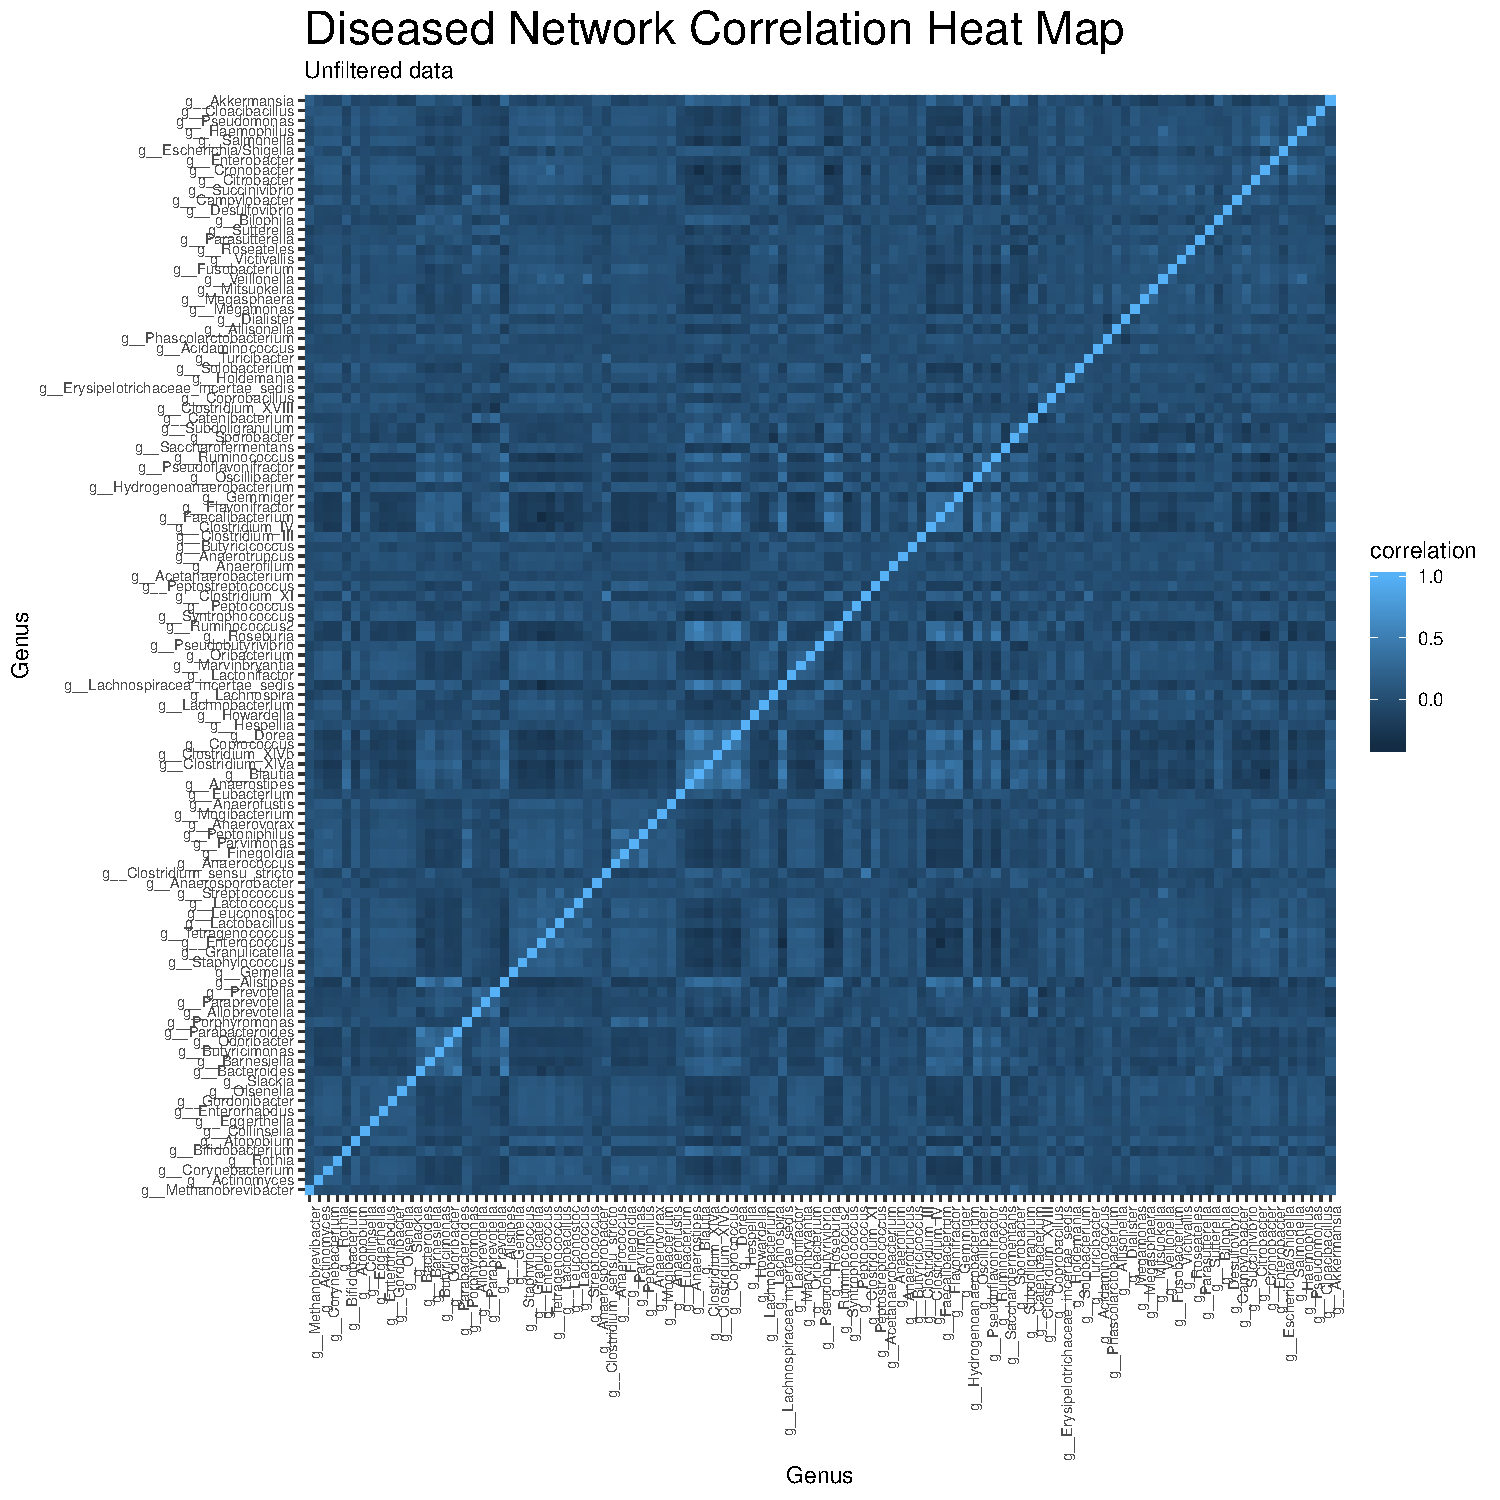
\includegraphics[width=1.0\linewidth]{figure/results/diseased_raw_corr_heatmap.pdf}
    \caption[Heat map of the resulting diseased FastSpar correlation matrix.]{Heat map of the resulting diseased FastSpar correlation matrix. Genera are listed on the respective axes and correlation values are colored based upon their strength. }
    \label{apdx-fig-d-orig-heatmap}
\end{figure}

\begin{figure}[htb!]
    \centering
    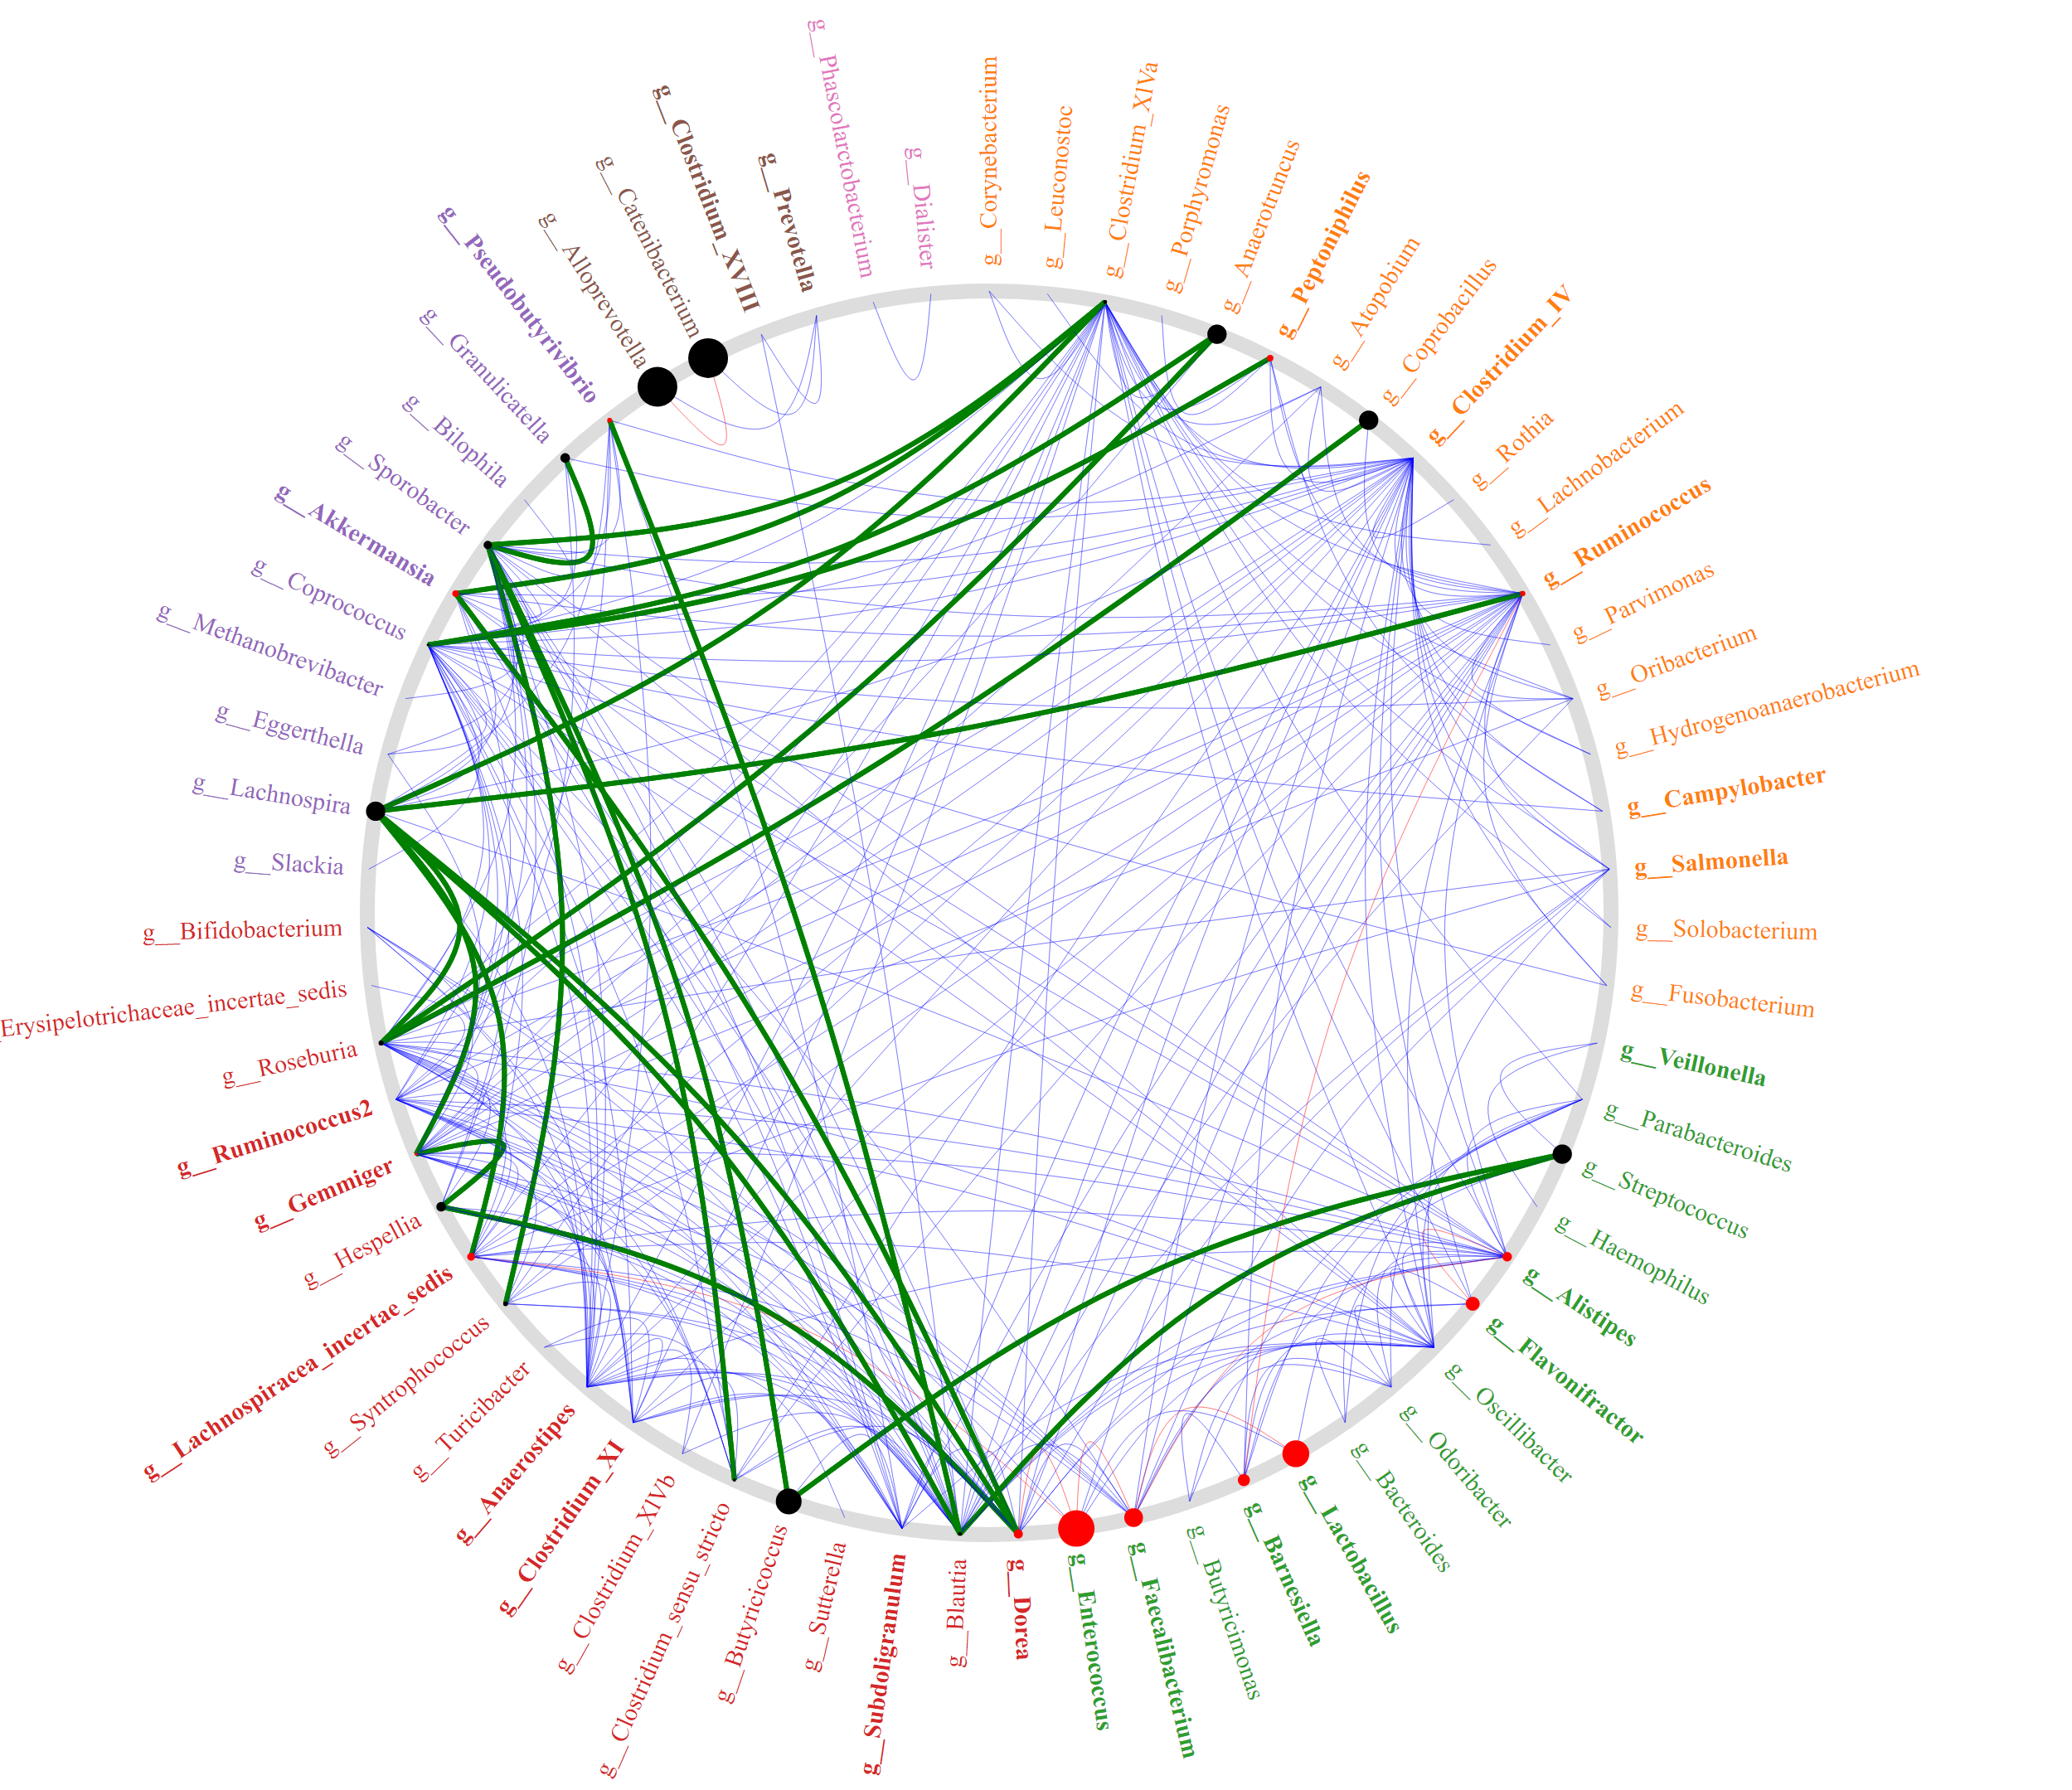
\includegraphics[width=1.0\linewidth]{figure/results/control_only.png}
    \caption[NetShift diagram depicting all edges in the sub-graphs with the control-only edges highlighted in green.]{NetShift diagram depicting all edges in the sub-graphs with the control-only edges highlighted in green. Genera are colored by their assigned sub-communities. Nodes are scaled by their \acrshort{NESH} scores, and nodes are colored red if they have been identified as important drivers. Control-only edges are in green, case-only edges are in red, and shared edges are in blue.}
    \label{apdx-fig-h-only-nesh}
\end{figure}

\begin{figure}[htb!]
    \centering
    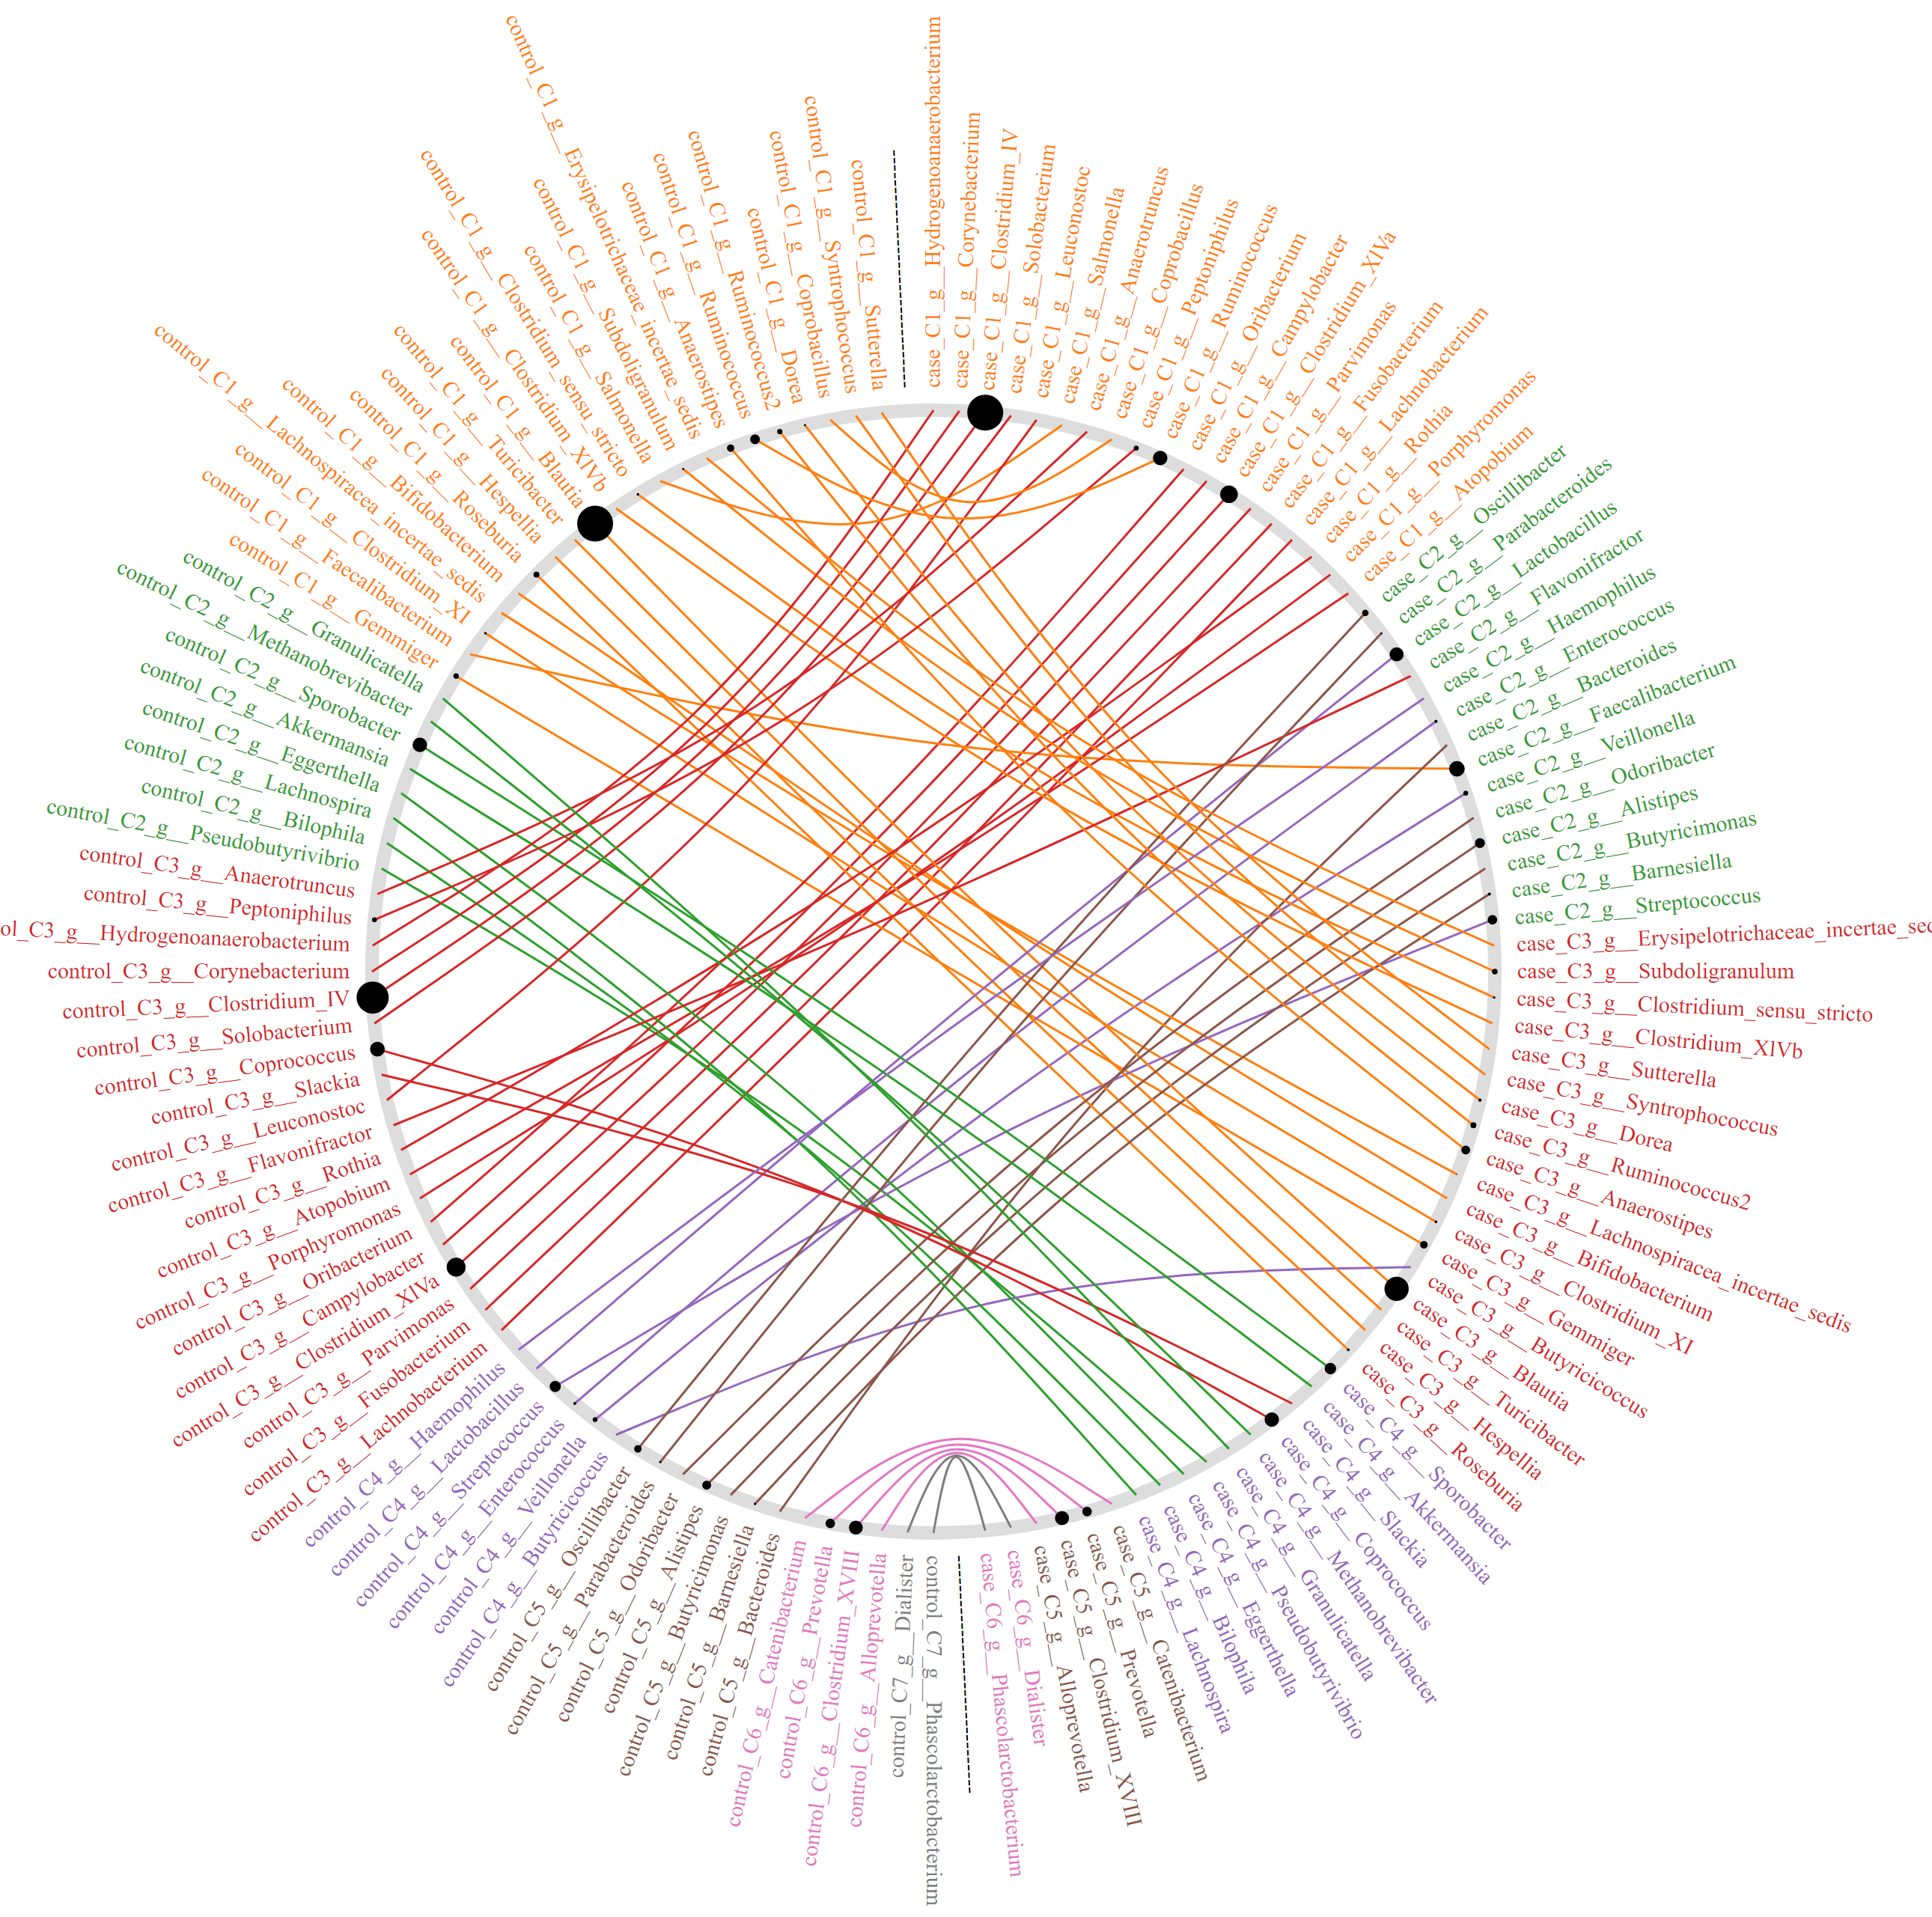
\includegraphics[width=1.0\linewidth]{figure/results/shuffle_net.png}
    \caption[The NetShift shuffle network diagram allows for the visual identification of taxa that change communities between the healthy (control) and diseased (case) networks.]{The NetShift shuffle network diagram allows for the visual identification of taxa that change communities between the healthy (control) and diseased (case) networks. All taxa are represented by the control taxa on the left of the diagram, and case taxa on the right. Communities are identified by the color of the taxa. Using the shuffle plot in Figure \ref{fig:res-shuffle} can be useful to interpret this diagram.}
    \label{apdx-nesh-shuffle}
\end{figure}
